\section{ SP0003GB23 }


\subsection{Meta}

    \textbf{Title:}
    Machine learning models to predict surgical case duration compared to current industry standards: scoping review

    \begin{table}[H]
        \centering
        \begin{tabular}{|c|c|c|c|c|c|c|c|c|c|}
            \hline
                \textbf{Rank} & \textbf{Grasp} & \textbf{Type} & \textbf{Output} & \textbf{Domain} & \textbf{COV19} & \textbf{CoI} & \textbf{DB} & \textbf{PR} & \textbf{Fnd} \\
            \hline
                5 & 94\% & A & P & A & Yes & No & Yes & Yes & No \\
            \hline
        \end{tabular}
        \caption{Reference's metadata}
        \label{tab:SP0003GB23}
    \end{table}

\subsection{Summary}
Christopher Spence et al. \cite{x084} published a narrative literature review of machine learning models for predicting surgery durations and challenged the standardised methods in the industry with machine learning algorithm efficiency. The authors searched studies on the open source databases till July 28, 2023. From 2593 publications, only 14 were accepted by the authors for in-depth analysis. The current work clearly states the paper selection process with a graphical flow visualisation. The analysis of the ML studies includes comparing the dataset size, data management, hospital implementation, model efficiency, model complexity and some fundamental construction differences in ML models. In conclusion, the authors highlighted the superiority of the ML models over standardised approaches and, at the same time, the need for more concrete ways of implementing and generalising the ML solutions in hospitals and the existing challenges to the researchers in the field of surgery duration prediction.
    

\subsection{Notes}
    \begin{itemize}
        \item Libraries: PubMed, Embase, MEDLINE, ClinicalTrials.gov, and the Cochrane Central Register of Controlled Trials (CENTRAL).;
        \item Frameworks: PRISMA, Arksey and O’Malley;
        \item Check out national audit office NAO for open data; 
        \item What is gray literature search;
        \item Medical Subject Heading (MeSH);
        \item Oxford Centre of Evidence-Based Medicine (OCEBM);
        \item Sources of data: 11, 16, 18-25, 39-42;
        \item National database: 19, 20, 40;
        \item Superior study in spectrum of sample size and explonation - 24;
        \item Data source EHR;
        \item What is retrospective observational study?
        \item What is randomized control trial?
        \item Contains details comparison table;
        \item TRIPOD-AI (59)?
        \item \href{https://academic.oup.com/bjsopen/article/7/6/zrad113/7343203#supplementary-data}{Supplementary materials;}
    \end{itemize}


\subsection{Reading}

    \textbf{Abstract:}
    The 2019 pandemic brings challenges to the scene of healthcare management. The novel AI approaches have been implemented in more rate. There is a question, whether the artificial intalligance approaches can substitute the existing healthcare standarts. The literature until July 2023 was selected and analysed.13 of 14 studies (2593 articles) demonstrate that machine learning is better than existing standardised approaches. NN is superiar to any other machine learning algorithm. The AI niche is surgery duration prediction, for more areas of application the further research is required.

    \textbf{Objectives:}
    Compare the novel machine learning approaches for predicting surgical case duration to present industry standards.
    
    \textbf{Page 1:}
    The consecuances of COVID-19 almost doubled the number of patients in waiting lists requiring surgery in 2023 compared to 2020. The national audit office (NAO) estimates plus four and a half million of cases by March  2025. There are mechanism to reduce waisted time. The empirical estimation of surgery duration by surgeons should be changed to more advanced approach to improve the operating theatre efficiency. There is no generalised solution. Here the authors introduce AI, ML, and DL.
    \begin{figure}[H]
        \centering
        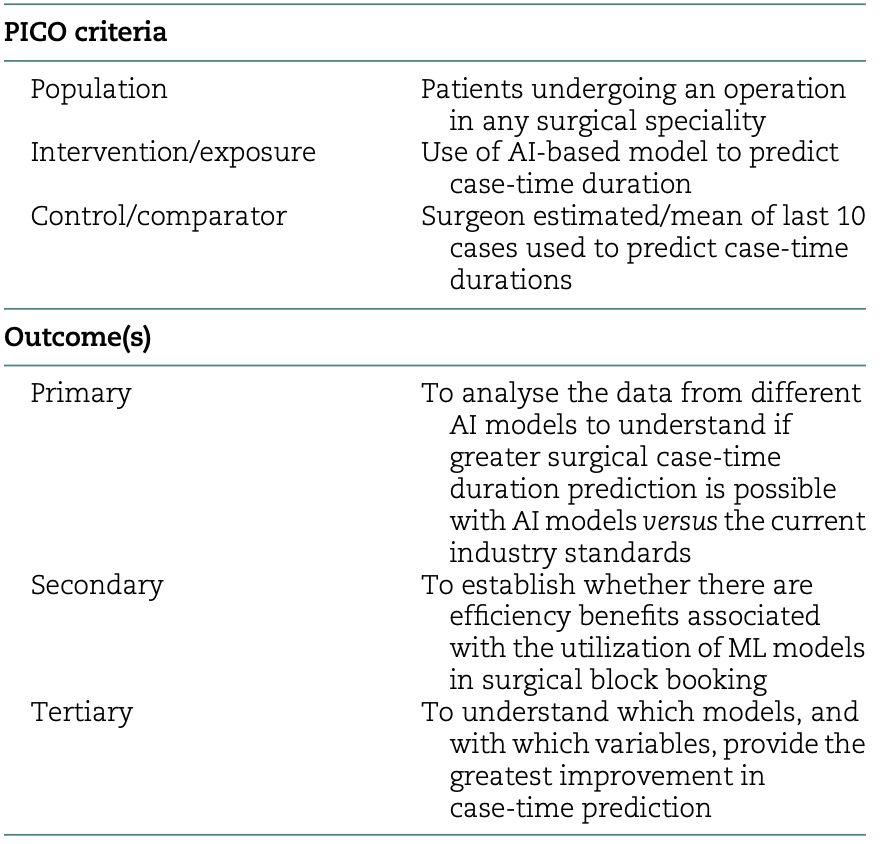
\includegraphics[width=.8\textwidth]{figures/SR0003GB23/fig1.png}
        \caption{PICO framework from \cite{x084}.}
        \label{fig1:SP0003GB23}
    \end{figure}
    
    \textbf{Page 2:}
    DL has more then 4 layers. DL is promising diraction for estimating the surgery duration, and it already has success in other healthcare scenarios. ML require accurate training dataset to produce efficient results. PRISMA protocole was developed for the literature scoping (can b accessed on request). Formulate research question: are AI approaches better?       
    The search on each database to 28 July 2023. The titles and anstractes screened separatly and disputes were sellted by seniour researcher.
    
    \textbf{Page 3:}
    The data was extracted from the publications and structured using MS Excel v14. The evidence assessment is conducted with Oxford Centre of Evidence-Based Medicine (OCEBM). Since the meta-analysis is not feasable, the narrative analysis was rendered instead. There are numerouse mathematical evaluational metrics for the literature resources. From 2593-initial-search result only 14 articles are fully following the requirements. Not all authors diclose their conflict of interests. The data management and documentation is not consistant throughout the studies. The explanation are more or less consistent with all 14 papers.
    11 Studies are from USA and the last three are from Canada, Colombia, and taiwaan. Dataset sizes vary from 500 to 302,300. The depth of the input data starts from seven and goas up to $>$1500. There is only one work which is done an external valisation of the DL model. The variaty of machine learning techniques was used in the overviewed submissions.
    
    \textbf{Page 4:}
    The factors with the most impact on the predictions are: surgery specialty, expert prediction, primary surgeon, patient weight, and average surgery duration. The all studies, with one exception, demonstrated comparison of multiple ML approaches. Efficiency savings are in the discussion section. Only one publication presented the time efficiency saving. The tree-based MLs show the most accurate predictions. The ML is not always worth then DL, but usually by increasing the training sample size, the DL eventually stay in lieder's position.
    \begin{figure}[H]
        \centering
        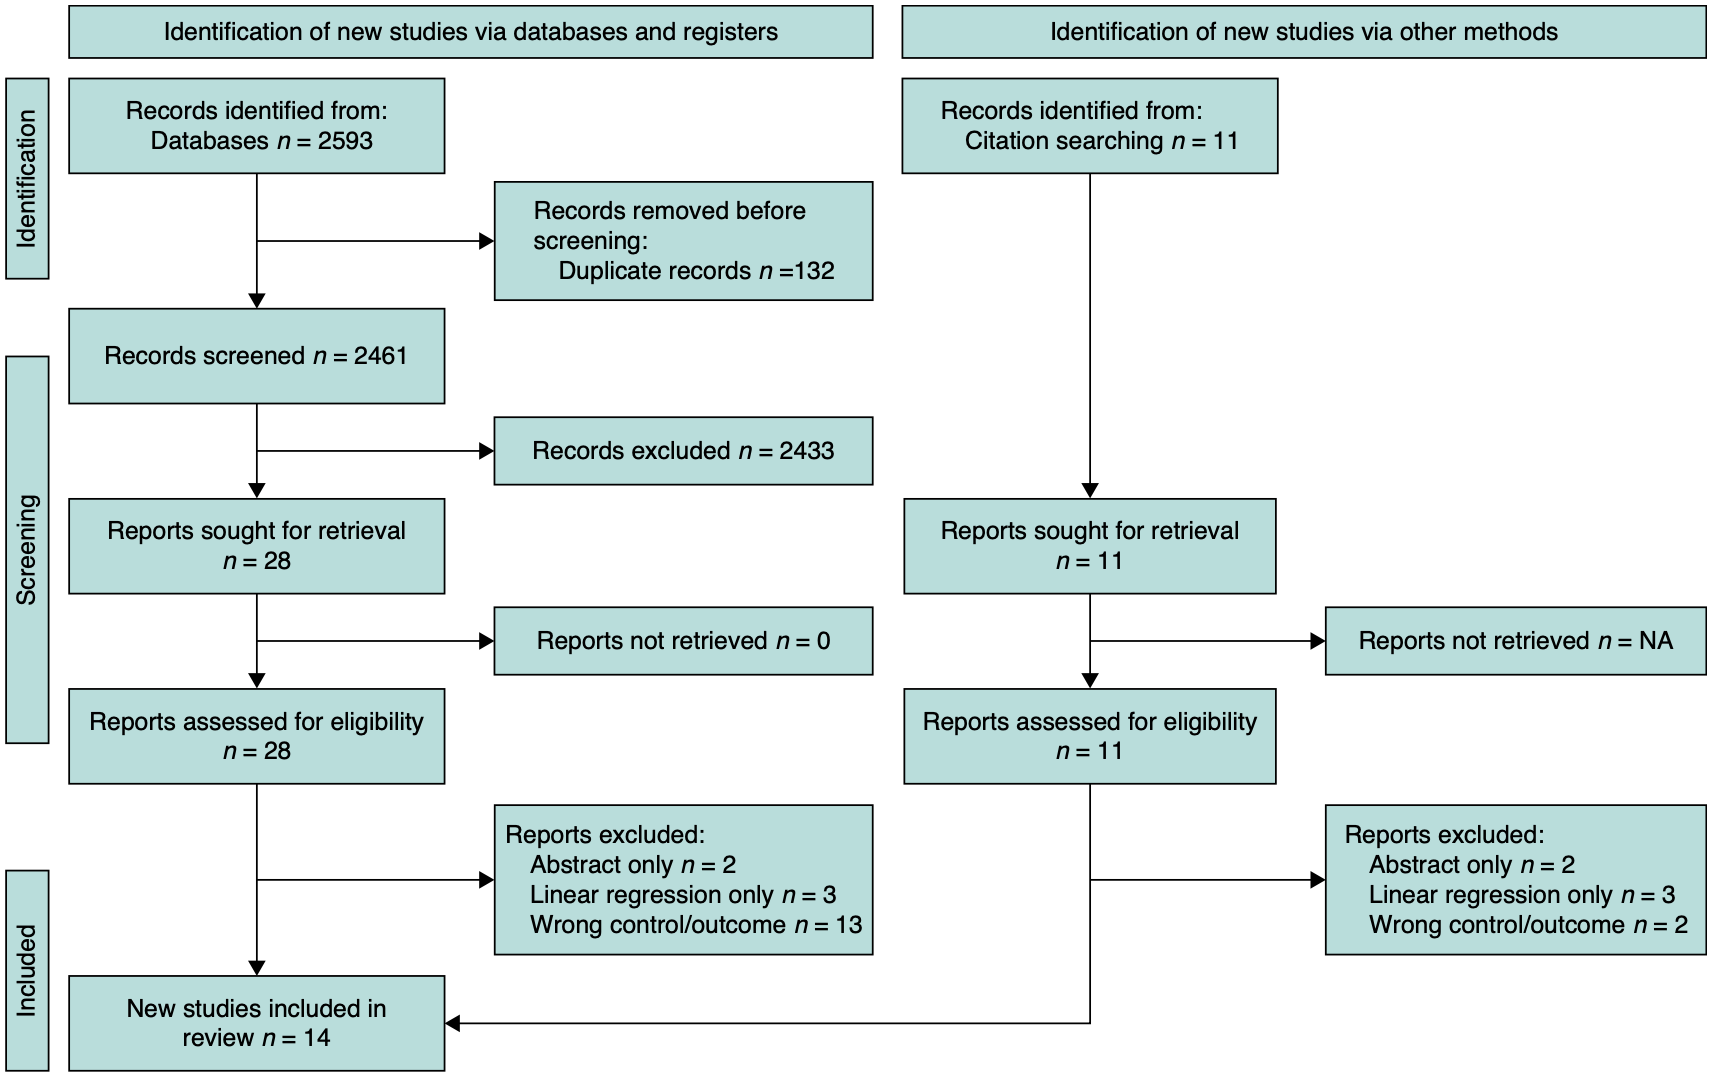
\includegraphics[width=1\textwidth]{figures/SR0003GB23/fig2.png}
        \caption{PRISMA diagram demonstrating the process of study selection, from screening to inclusion and the grey literature search (created using the online tool of Haddaway et al. (38)) from \cite{x084}.}
        \label{fig2:SP0003GB23}
    \end{figure}
    
    \textbf{Page 5:}
    The authors describe in more detail work by Jiao et. al. (19). The most common critarias: 
    \begin{itemize}
        \item primary surgeon, 
        \item historic average surgical duration, 
        \item the experience of the surgeon, 
        \item procedure name, 
        \item the number the procedure lies within the list, 
        \item type of anaesthesia,
        \item duration of the case, 
        \item patient BMI, 
        \item patient age, 
        \item ASA score, 
        \item patient sex, 
        \item patient co-morbidities,
        \item anaesthesia provider (consultant/junior).
    \end{itemize}
    The clearing the medical records from redandant critarias helps reduce noise. Also, quality of the recording metters to the prediction outcome. ASA has lower importance than patient weight. Specific case of ML failure for correct prediction. The large predictions errors can significantly disrupt the hospital flow. Average OT costs in USA fluctuates from \$22 to \$133. The ML tend to ignore overruns in the surgery duration prediction. Abbas et al. (40) managed data in a way that provided generalise approach for the USA. The cleaning of datasets with missed fields have not been addressed in several studies. It is not enought to train on the dataset less then 1000, and large datasets is a must. There are numerous publications which are probably not generalisable.
    
    \textbf{Page 6:}
    There is sparce number of ML implementations. There are only 14 accepted studies which may indicate challange to conduct sufficient scientific report in this field. The implementation and maintanance of the ML models require coordination from parties with divarce background. The AI policy is not evolved enough. There are requirements for efficient ML usage, such as tachnical aspects and motivated human resources. Also the surgery duration prediction is not the only way of applying ML. Raising multiple general musts. The ML/DL are more optimal way of the surgery duration prediction, but there is not enough work done for proper injection of the technology into hospital's workflow. The authors provide the authors' contribution section.